\documentclass[plutus.tex]{subfiles}
\begin{document}
\section{Applications: the \glsentrylong{paf}}
\label{sec:paf}

An application that interacts with the blockchain is some kind of program that runs on a users computer.
But what does that application actually do?

For starters, \glspl{app} that make use of the ledger's scripting functionality will need to create appropriate \gls{plutus-core} programs.
We discuss how we enable this for Haskell applications in \cref{sec:plutus-tx}.

However, even very simple applications have some clear needs.

Consider one of the simplest possible \glspl{app}:

\paragraph{Metadata Poster}
Metadata Poster does nothing except occasionally submit transactions to the chain.
The transactions which it submits do not move any substantive amount of value, their purpose is just to post a transaction to the chain with some metadata payload that can later be checked by another application.\footnote{
This may seem like a silly example, but many real proposed applications in supply-chain management are essentially just Metadata Poster!
}
\medskip

Firstly, Metadata Poster needs to communicate with a number of other components:
\begin{itemize}
\item It needs to submit transactions, so it must talk to a \gls{node} or a \gls{wallet-backend}.
\item It needs to acquire funds to pay fees, so it must talk to a \gls{wallet-backend}.
\item It must talk to its users, so it must expose some kind of API or talk to a graphical interface like a \gls{wallet-frontend}.
\end{itemize}

Moreover, Metadata Poster may care about some of the rollback issues discussed in \cref{req:app-rollback}.

Finally, there are a number of operational issues common to \glspl{app}:
\begin{itemize}
\item It may need to be distributed to end users and receive updates.
\item It may need to synchronize its state between multiple instances (e.g. desktop and mobile).
\item It may need to have its state backed up by systems administrators.
\item It may need to provide logging and monitoring for production usage.
\end{itemize}

It is clear that there is a lot of complexity in the \gls{off-chain} part of a \gls{app}.
Enough that we probably cannot simply leave this in the hands of application developers.
The \glsfirst{paf} is our response to this problem: a disciplined framework for writing \glspl{app} that eases many of these problems.

\begin{figure}[t]
  \centering
  % Source: https://docs.google.com/drawings/d/19BtPqP9mbRQr_zqrzImLRnTeMMvTgH6betGPleDlWzg/edit
  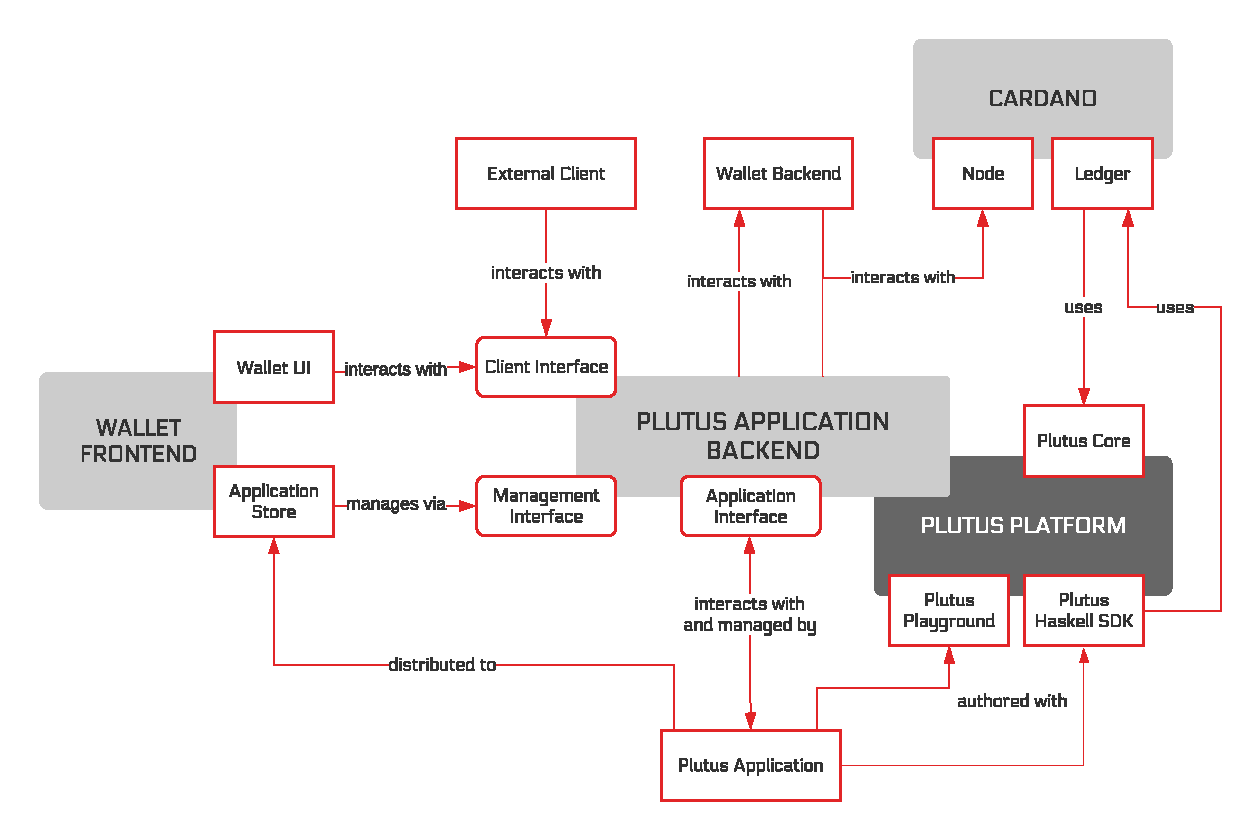
\includegraphics[width=\textwidth]{paf-architecture.pdf}
  \caption{Architecture of the \gls{paf}}
  \label{fig:paf-architecture}
\end{figure}

\subsection{Requirements}
\begin{requirement}[Backups]
\label{req:app-backups}
\Glspl{app} need to be easy to back up, if they are to be used in production.
\end{requirement}

\begin{requirement}[Monitoring]
\label{req:app-monitoring}
\Glspl{app} need to be easy to monitor, if they are to be used in production.
\end{requirement}

\begin{requirement}[Synchronization]
\label{req:app-synch}
It should be possible to synchronize the state of an \gls{app} between instances on multiple machines, e.g. a mobile and a desktop instance.
This is quite important for consumer-type users.
\end{requirement}

\begin{requirement}[Reproducibility]
\label{req:app-reproducibility}
\Gls{app} behaviour should be reliable and reproducible on different environments and devices.
For example, \glspl{app-inst} that have had their state synchronized (\cref{req:app-synch}) should behave identically.
\end{requirement}

\begin{requirement}[Distribution]
\label{req:app-dist}
\Glspl{app} need to be distributed to users somehow.
Different users may have different needs here, for example:
\begin{itemize}
\item A consumer user may want to download an \gls{app} from a centrally managed ``app store'' in their \gls{wallet-frontend}.
\item A business user may want to download a native application via their usual package manager, or directly from the author.
\end{itemize}
\end{requirement}

\begin{requirement}[Flexible, self-describing application endpoints]
\label{req:app-client-interfaces}
\Glspl{app} will want to expose endpoints to users which trigger the functionality of the application.
These need to be accessible to both server-side headless consumers, and also to graphical \glspl{wallet-frontend} which mediate interaction with end-users.

Ideally, these endpoints would be \emph{self-describing} so that we can have at least basic generic interfaces in e.g. a \gls{wallet-frontend}.
\end{requirement}

\begin{requirement}[Chain data access]
\label{req:app-chain-data}
\Glspl{app} need to access some historical data about the chain.
In particular, due to \cref{req:ledger-utxo-size} the \glspl{datum} for \glspl{script-output} are not stored in the \gls{utxo} set, but rather in the transaction that creates the output.
\Glspl{app} will need to know about these \glspl{datum}, so we must provide some way of tracking this information from the chain and making it available.

\todompj{Should link to wherever we discuss the whole issue with storing datums in detail.}
\end{requirement}

\begin{requirement}[Rollback resistance]
\label{req:app-rollback}
Rollbacks can cause serious problems for agents (not just applications) trying to take conditional actions.
It would be nice if we could mitigate these for \glspl{app}, but that may not always be possible.

Here are two scenarios we might care about.

\paragraph{Incoherent choice}
\label{para:incoherent-choice}
Suppose that Alice promises to send 10 \gls{ada} to Bob, provided that Bob sends 20 \gls{ada} to Carol (perhaps Alice is holding Bob's collateral for a loan from Carol, which Bob is now repaying).
The following events occur:
\begin{enumerate}
\item Bob pays 20 \gls{ada} to Carol in transaction T1.
\item Alice observes T1, and proceeds to pay 10 \gls{ada} to Bob in transaction T2.
\item A rollback occurs. After the rollback, T1 and T2 go back into the mempool, but T1 is now invalid.
\item T2 alone is reapplied.
\end{enumerate}

As a result, Alice ends up making the payment to Bob without Bob paying Carol, so Bob gets away with all the money!
Alice ends up committed to an action that she would only have chosen to do the old history of the chain, and which she would not have chosen to do the new history.

\paragraph{Incomplete reapplication}
\label{para:incomplete-reapplication}
Suppose as a variant of the previous scenario that Alice promises to send 10 \gls{ada} to both Bob and Carol, provided that some off-chain event happens.
The following events occur:
\begin{enumerate}
\item The off-chain event occurs.
\item Alice pays 10 \gls{ada} to Bob in transaction T1.
\item Alice pays 10 \gls{ada} to Carol in transaction T2.
\item A rollback occurs. After the rollback, T1 and T2 go back into the mempool, but T1 is now invalid.
\item T2 alone is reapplied.
\end{enumerate}

As a result, Alice ends up only paying Carol and not Bob.
Alice ends up \emph{partially} taking an action that she still wants to take, and would need to reconstruct the missing parts to get back to the state she wants to be in.
\end{requirement}

\begin{requirement}[Testing and emulation]
\label{req:app-emulation}
Users need to be able to test their \glspl{app} in an environment that mirrors the real one as closely as possible.
However, the real environment is very complex, featuring a multi-agent, distributed system with a number of tricky behaviours: network issues, rollbacks etc.

It is therefore desirable to provide some kind of emulated testing harness which users can use to test their \glspl{app} locally, but which allows control and simulation of real issues.

Moreover, this is important for us during development, as it allows us to mock up the system that we expect without having to wait for other components to be ready.
\end{requirement}

\subsection{Lifecycle of a \glsentrytext{app}}

The lifecycle of a \gls{app} is as follows:

\begin{itemize}
\item
  \Glspl{app} are authored and compiled with the \gls{plutus-sdk} using the \gls{app-api} for interacting with other components.
\item
  \Glspl{app} are distributed via some means to be decided, but manually in the interim.
\item
  \Glspl{app} are installed into an instance of the \gls{pab}. The \gls{pab} just knows about the compiled \gls{app-exe} provided by the \gls{app}.
\item
  A \gls{app} can be instantiated into a \gls{app-inst} by running the \gls{app-exe} and providing any parameters that it needs.
  There can be multiple \glspl{app-inst} per \gls{app}, and they are managed by the \gls{pab}.
\item
  The \gls{pab} manages and handles the requirements of the \gls{app-inst} throughout its lifecycle, including interaction with external clients such as \glspl{wallet-frontend}.
\end{itemize}

The major component here is the \gls{pab}.

\subsection{The \glsentrylong{pab}}
\label{sec:pab}

\fbox{
\begin{minipage}{\textwidth}
WARNING: this component is under heavy development, so this will likely evolve and may not represent the current state of things.
\end{minipage}
}
\medskip

A key component of the \gls{paf} is the \glsfirst{pab}.
This is a backend service (like the \gls{wallet-backend}) that intermediates between \glspl{app}, the \gls{node}, the \gls{wallet-backend}, and users (including the \gls{wallet-frontend}).

The \gls{pab} will be run in similar contexts to the wallet backed, e.g. backing a graphical user wallet (e.g. \gls{daedalus}), or on a server that runs \glspl{app} as part of a larger system.

The purpose of the \gls{pab} is to:
\todompj{Do this in prose? Also all the provisions here should be expanded and moved to requirements}
\begin{itemize}
\item Provide a standardized environment for \glspl{app} to run in (\cref{req:app-reproducibility,req:app-monitoring})
\item Provide disciplined state management (\cref{req:app-backups,req:app-synch,req:app-rollback})
\item Present discoverable interfaces to the external clients (\cref{req:app-client-interfaces})
\item Track information from the chain for use by contracts (\cref{req:app-chain-data})
\item Work in an emulated environment (\cref{req:app-emulation})
\end{itemize}

The \gls{pab} is a series of components which produce/consume events, and a message bus.

Some of the components have additional complexity, e.g. the application management component needs to manage the state of \glspl{app-inst}.

\subsubsection{Node client}
The \gls{pab} needs to talk to the \gls{node}, primarily because it needs to populate the \gls{chain-index}, but it may also need to do some things that appear to be the \gls{wallet-backend}'s job (e.g. maintaining pending sets), because we can't guarantee that the \gls{wallet-backend}'s view of the world will match our own (since each is independently talking to the \gls{node}).

\subsubsection{\Glsentrytext{wallet-backend} client}

The \gls{pab} needs to talk to the \gls{wallet-backend} for a number of things:
\begin{itemize}
\item Coin selection/transaction balancing
\item Transaction signing and submission
\item Address creation
\end{itemize}

You might think that since the \gls{pab} has a node client itself, it could do its own transaction submission, and only rely on the \gls{wallet-backend} for signing.
However, transactions made by the \gls{pab} will likely use outputs ``owned'' by the \gls{wallet-backend} (e.g. those selected by coin selection from the user's outputs).
Hence it is important that the \gls{wallet-backend} knows about such outputs, so that it does not attempt to spend them somewhere else.

\subsubsection{Event system}

The \gls{pab} needs to handle incoming events from a number of sources concurrently, so we need some kind of message bus.
In addition, the persistence story for \glspl{app-inst} involves persisting their incoming events, so this is a good fit.

We are currently using an event-sourced architecture here.
We hope that this will make backups and synchronization easier (\cref{req:app-backups,req:app-synch}).

\subsubsection{Application management}

\Gls{app-inst} need to be managed, created, destroyed, fed with events, etc.

\begin{itemize}
\item Create \glspl{app-inst}
\item Instantiate and run \glspl{app-exe} in a sandbox
\item Handle communication with the \gls{app-exe}
\item Handle own message queue (``mailbox'') for each \gls{app-inst}
\item Manage/dump/load \glspl{app-inst}
\item Create/destroy \glspl{app-inst}
\item Handle rollbacks
\end{itemize}

\subsubsection{\Glsentrytext{chain-index}}

Applications need to access \glspl{datum} for outputs (see \cref{req:app-chain-data}), so we need some kind of system that monitors the chain and records (at least) the \glspl{datum}.

\subsubsection{Client interface}

For external clients (other programs), including graphical \glspl{wallet-frontend} to talk to.
Should expose some of the application endpoints and \gls{app-inst} management functionality.

\subsubsection{Logging and monitoring}

To satisfy \cref{req:app-monitoring}.

\subsection{Emulators}

In order to satisfy \cref{req:app-emulation}, we need to write emulators for quite a number of components.

At present, we have (or expect to have) emulators for:
\begin{itemize}
\item
  The \gls{node} using our ledger extensions.
  In the long run we should be able to use the real Goguen \gls{node}.
\item
  The parts of the \gls{wallet-backend} that we need.
  In the long run we \emph{might} be able to use the real \gls{wallet-backend}.
\item
  Basic \gls{wallet-frontend} functionality, such as displaying balances and interacting with \glspl{app-inst}.
  In the long run we \emph{might} be able to use the real \gls{wallet-frontend}, but this seems unlikely as it is quite heavyweight.
  Having our own component here has the advantage that we can reuse it in the \gls{plutus-playground}.
\end{itemize}

We also need libraries to bind all of these into an overall, multi-agent simulation, and to allow users to write tests that exercise particular series of events in this simulation.

\subsection{The \glsentrytext{plutus-playground}}
\label{sec:plutus-playground}

The \gls{plutus-playground} provides a Web environment for getting started with the \gls{plutus-platform}.

The authoring experience in the \gls{plutus-playground} is fairly limited (one file only), but it has the best support for specifying ad-hoc scenarios and visualizing the results.

Over time we hope to unify the experiences of working locally and working in the \gls{plutus-playground}, by:
\begin{itemize}
\item Improving the authoring experience in the \gls{plutus-playground} (multiple files etc.)
\item Improving the visualization experience locally (sharing components with the \gls{plutus-playground})
\item Allowing distribution of simple \glspl{app} directly from the \gls{plutus-playground}.
\end{itemize}

\subsection{Application design}

\todompj{Talk about state machines and our ideas for handling rollbacks.}

\end{document}
